\documentclass{article}
\usepackage{graphicx}
\usepackage[utf8]{inputenc}
\begin{document}
\section{TP1 : Outil de simulation de réseaux : NS-2}
    \subsection{Exercice 1}
        L'interface graphique de 'nam' limite certain paramétrage comme par exemple la "Bandwidth" du CBR.
        %{# Screenshot #}
        Les options sur l'interface de nam sont limitées, ainsi, celle-ci est facile à prendre en main. Des boutons permettent de contrôler l'écoulement du temps dans la simulation, d'autres permettent d'agrandir et de réduire la vue pour se concentrer sur des parties spécifiques du réseau. Un slider permet d'ajuster le temps entre chaque étapes de la simulation.

        Nam dispose aussi d'un interface qui permet de simuler un scénario de façon graphique. Celle-ci comporte les fonctions de base sous forme de menu déroulant, permettant d'ajouter des noeuds, des connexions et des agents. Un clic droit permet d'ajuster les paramètres des éléments ajoutés.
        Certains réglages restent cependant inaccessibles, par exemple, la bande-passante du trafic CBR ne peut pas être ajustées afin de correspondre à ce que le script demande.
    \subsection{Exercice 2}
        On souhaite simuler un réseau constitué de 4 noeuds, tel qu'illustré dans le fascicule de l'exercice. On organise notre script afin de pouvoir efficacement corriger les éventuelles erreurs qui pourraient apparaître. On choisit de l'organiser de façon semblable au modèle OSI, on fragmente les lignes en fonction de la couche dont elles traitent.
        Les commandes permettant d'orienter les connexions entre les noeuds, ainsi que celle permettant de colorer un flux contribuent à rendre le résultat lisible, en dépit de la superposition des segments et des datagrammes.

    \subsection{Conclusion}
        Le TCP permet de gérer la perte de paquet (en gérant la congestion) contrairement à UDP.
        On utilise deux méthode pour savoir si un paquet à été perdu : "Timeout" et "3 Ack duplicate".
        
\section{TP2 : Outil de simulation de réseaux : NS-2}

    \subsection{Exercice 1: Protocoles de Routage}
    \subsubsection{Etablissement du réseau}
      On commence par réaliser le réseau demandé. Grâce au TP précédent, cela se fait rapidement, et selon les spécifications du sujet. On organise le code de la même façon que dans le TP précédent, pour plus de clareté. Le but de ce TP est de comparer les différences en termes de convergence, mise à jour de routage, et du comportement autour du noeud n5 de deux protocoles de routage, à Vecteur de distance et à Etat de lien. En ne changeant que ce facteur lors de 2 simulations, on pourra, à l'aide des outils fournis dans nam, facilement distinguer ce qui advient des paquets en transit pendant la perte de connexion, et comment les différents noeuds du réseau communiquent afin de réaliser le routage.
    \subsubsection{Vecteur Distance}
      On peut voir les captures d'écran dans les figures 2 à 6. Lors de la rupture, les paquets sont perdus, et le reroutage se met en route au bout de 30 ms. Lorsque la jonction est rétablie, le routage initial, plus court (dans les termes choisis par ns2) reprend lieu au bout de 10ms. Le protocole à Vecteur de Distance nécessite l'envoi de paquets périodiques (2s dans ns2) afin de maintenir le routage à jour, mais aussi lors du changement d'une distance au sein du réseau. Il s'agit donc d'une convergence lente.
    \subsubsection{Etat de liens}
      On peut voir les captures d'écran dans les figures 7 à 11. Lors de la rupture, cette fois-ci, les paquets ne sont pas perdus, ils sont simplement reroutés dès que possible, c'est-à-dire, quand une route est trouvée, au bout de 10ms (plus rapide qu'avec le protocole DV). Lorsque la jonction est rétablie, le routage reprend sa forme initiale, puisque plus rapide, et les paquets transitent comme avant la rupture au bout de 10ms. Ce protocole ne nécessite pas l'envoi de paquets périodiques, et pèse donc moins sur la congestion du réseau, par contre il nécessite l'envoi de paquets à chaque changements d'état d'une jonction. Étant plus rapide que le porotocole DV, on peut dire qu'il s'agit ici d'une convergence rapide.
    \subsection{Exercice 2: Routage et contrôle de congestion TCP}
      On réalise le réseau demandé, selon les spécifications précisées. On trace la courbe d'évolution de la fenêtre TCP (figure 1) en fonction du RTT, on précise la valeur de ssthresh et rwnd, et on détaille le nom des phases de l'évolution.
      
      Contrairement à l'exercice 2 du TP1, où il y avait de la congestion dû à trop de demandes d'utilisation du réseau, ici, une liaison est coupée. Il pourrait aussi y avoir des collision si le réseau était organisé différemment, causant la perte de paquets TCP.
      
    \begin{figure}
    \centering
    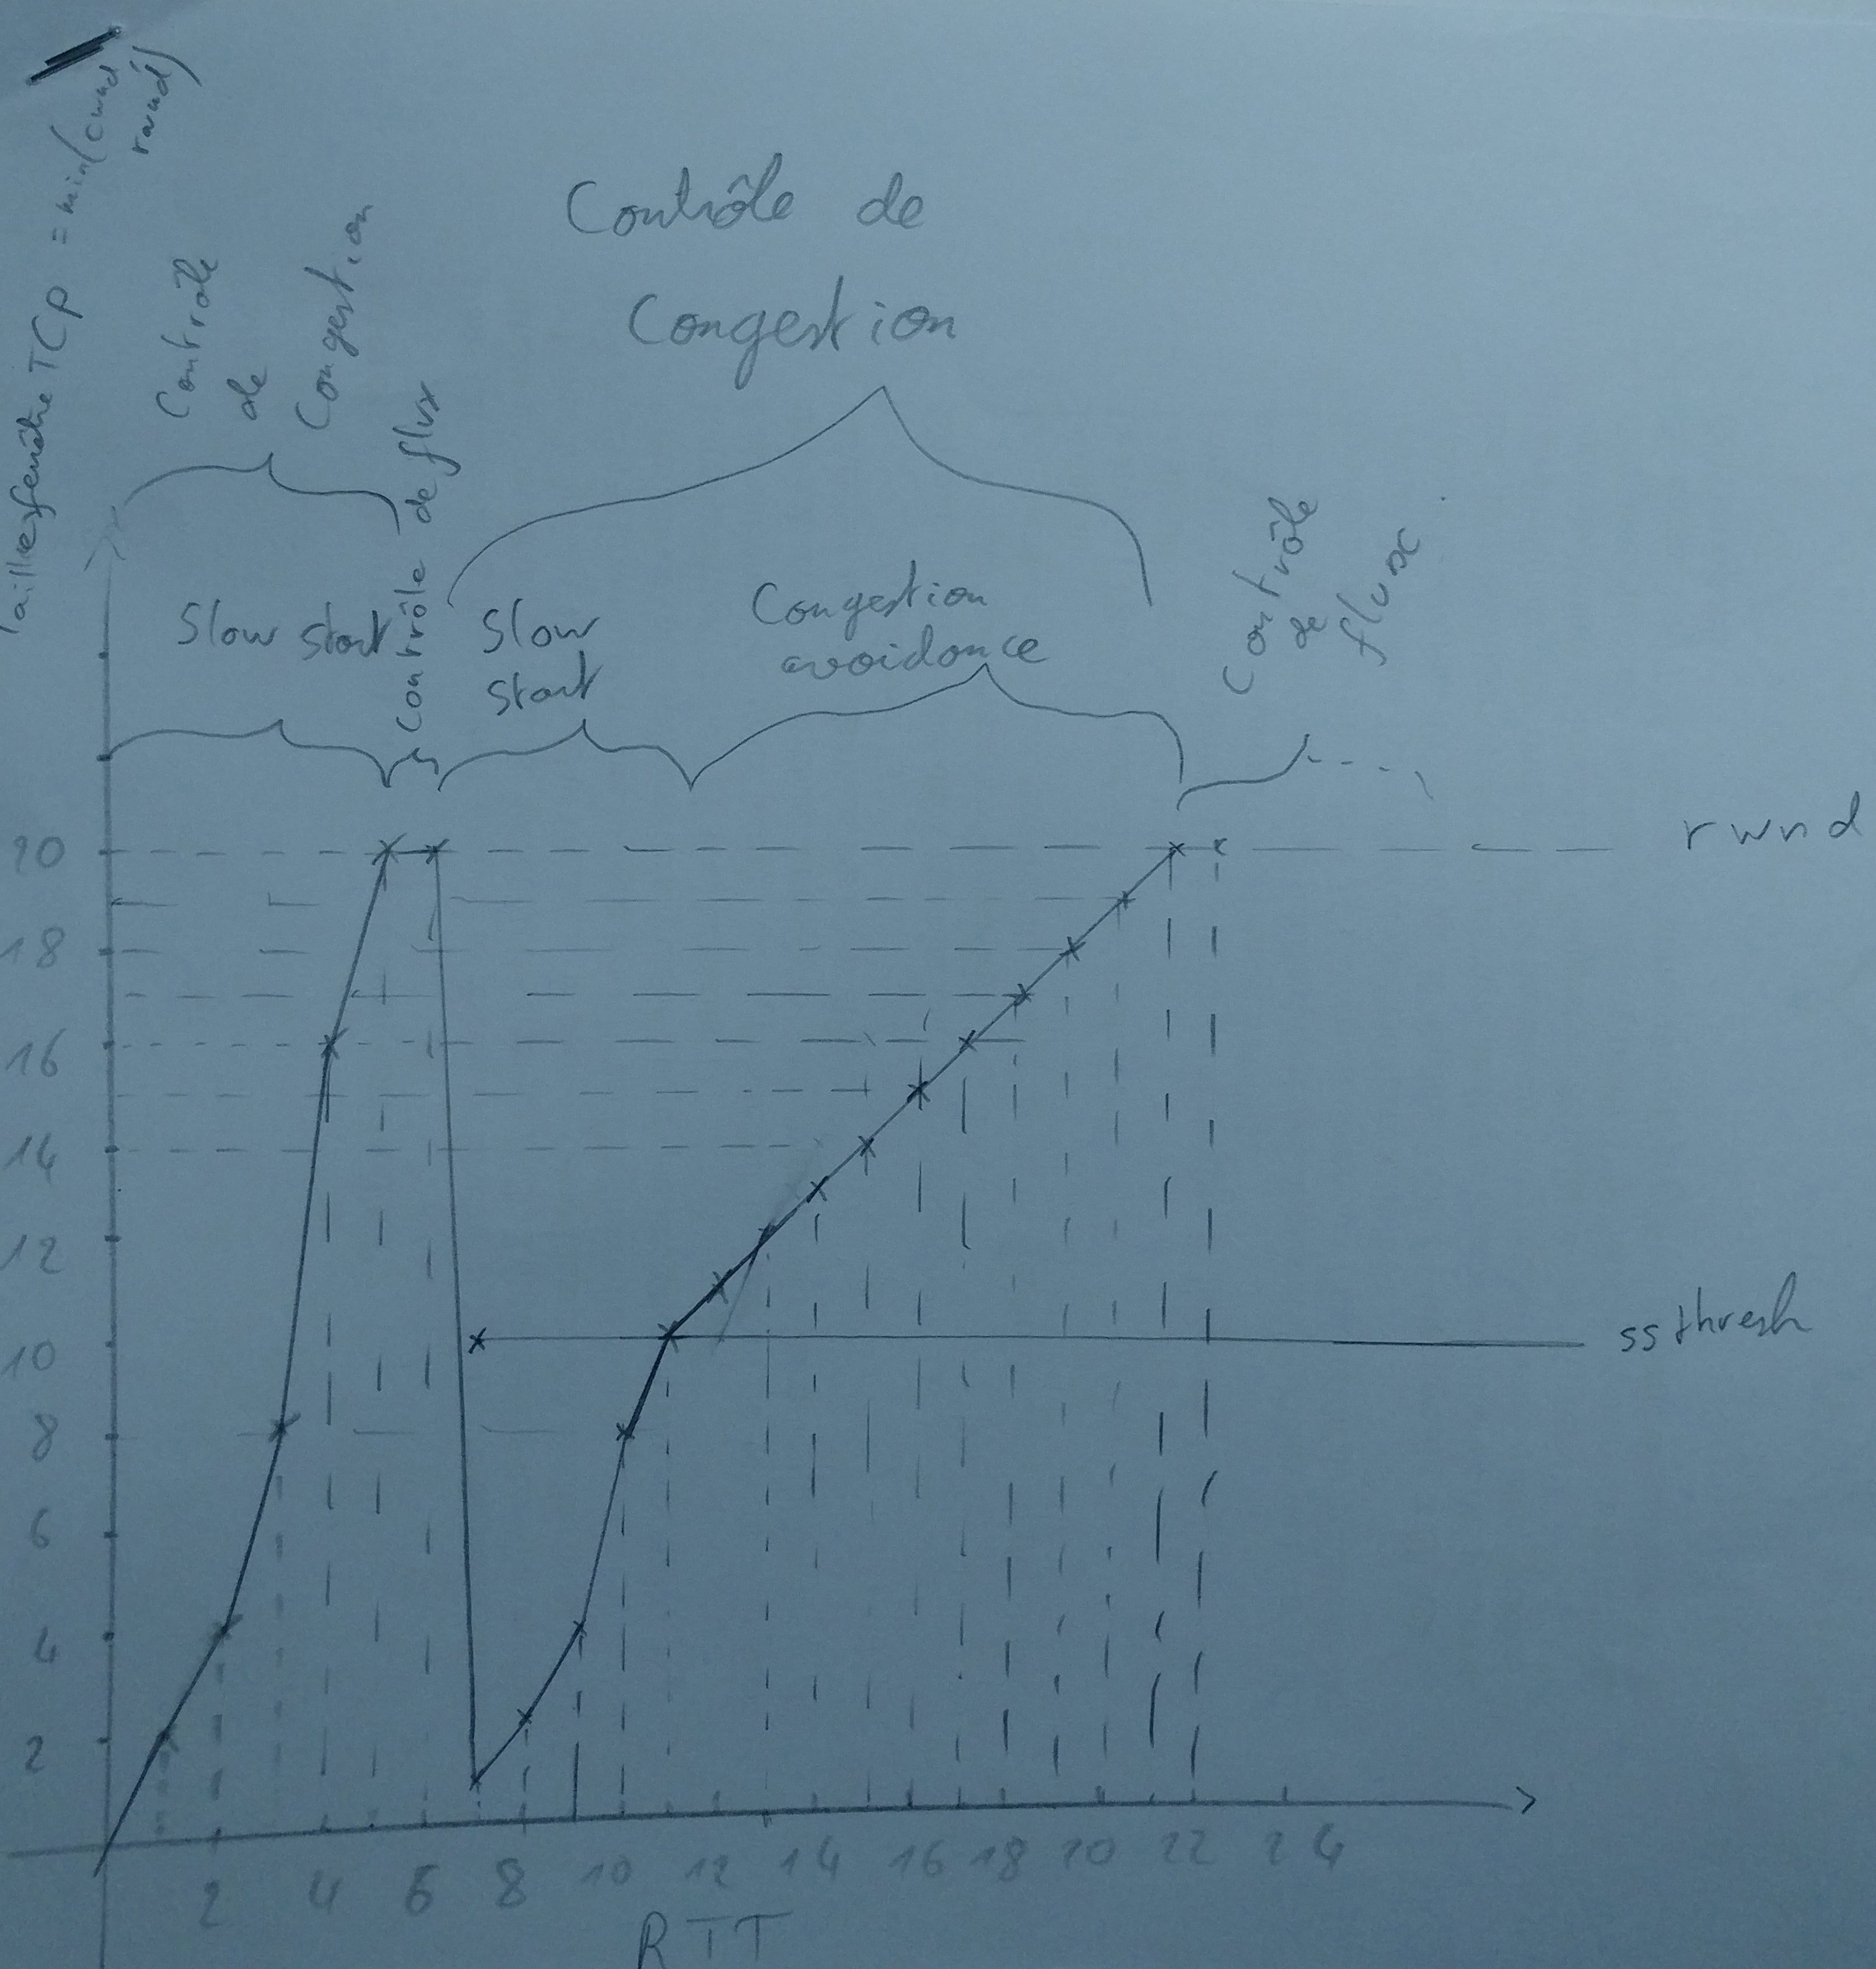
\includegraphics[width=0.99\columnwidth]{courbe.jpg}
    \caption{Courbe d'évolution de la fenêtre TCP en fonction du RTT}
    \end{figure}
    \vskip1ex
    \begin{figure}
    \centering
    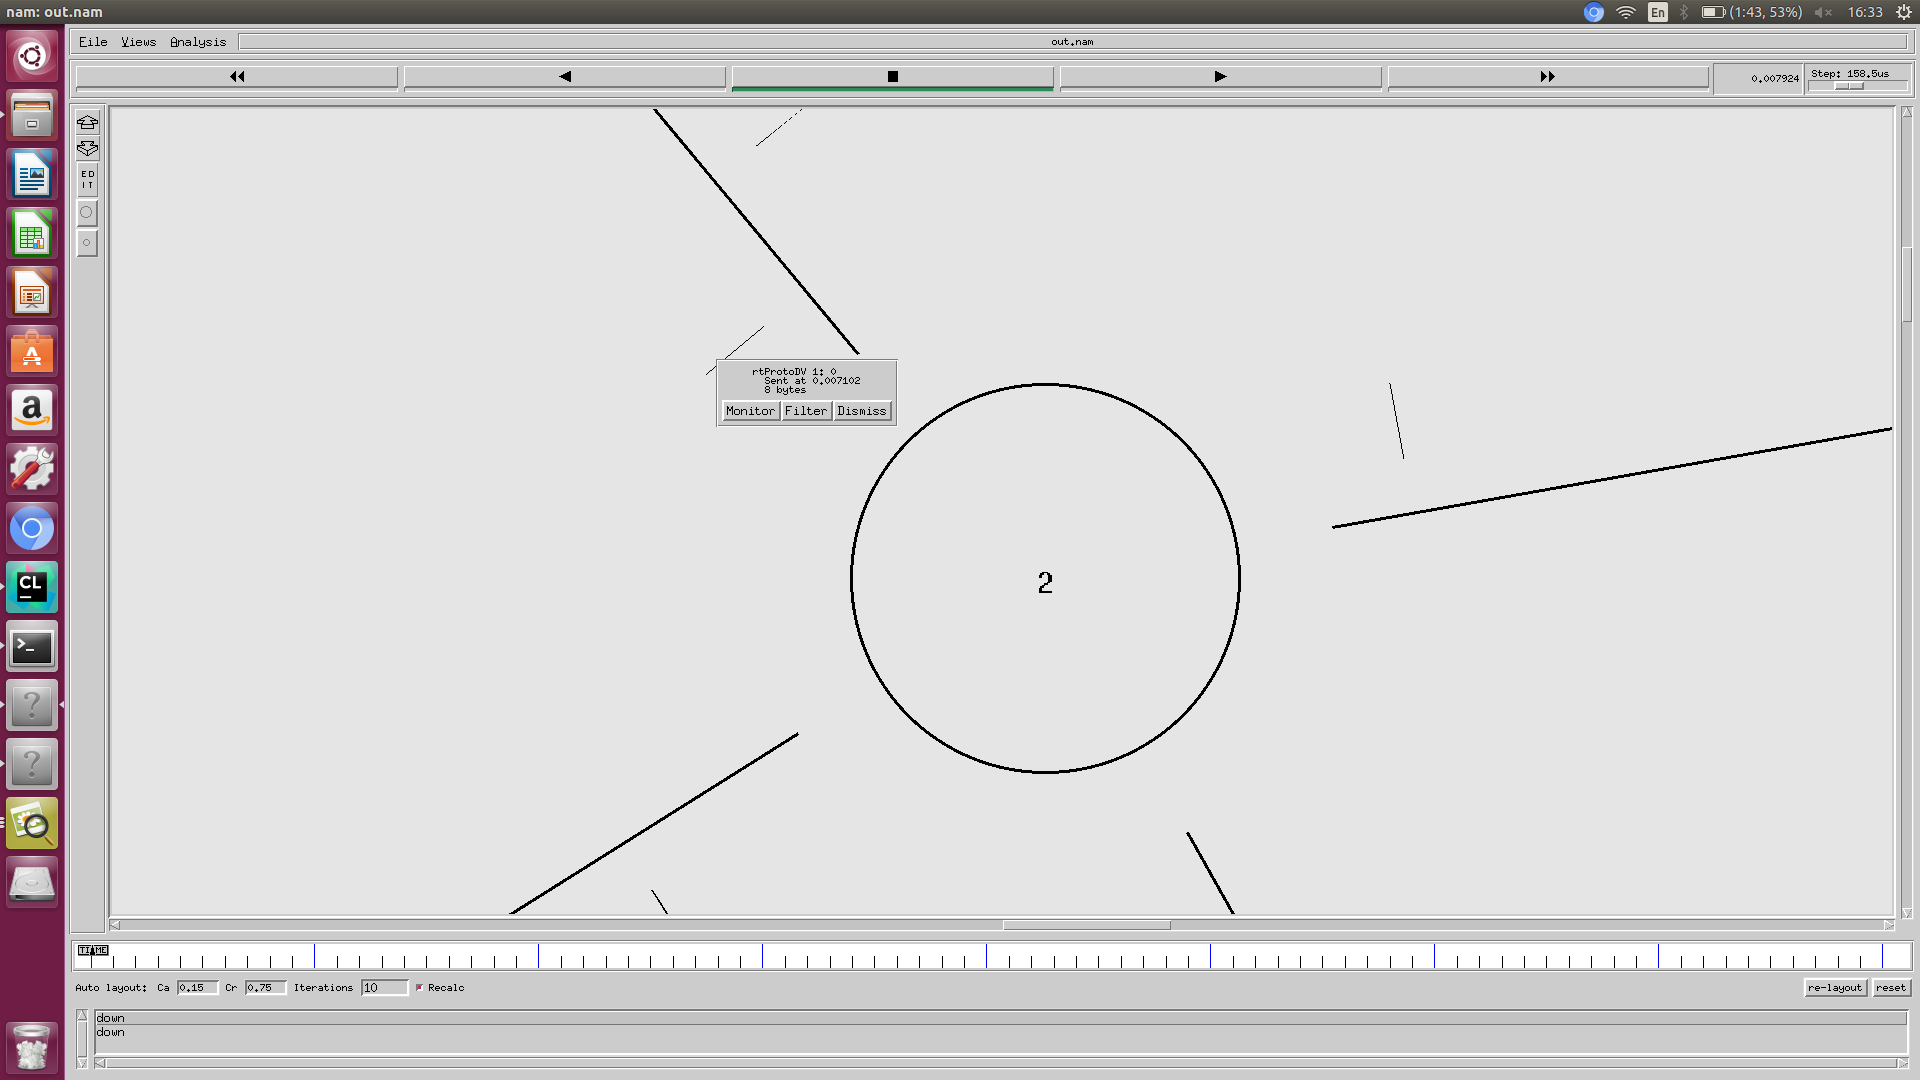
\includegraphics[width=0.99\columnwidth]{tp2-1-DV-1-init.png}
    \caption{Initialisation du routage}
    \end{figure}
    \vskip1ex
    \begin{figure}
    \centering
    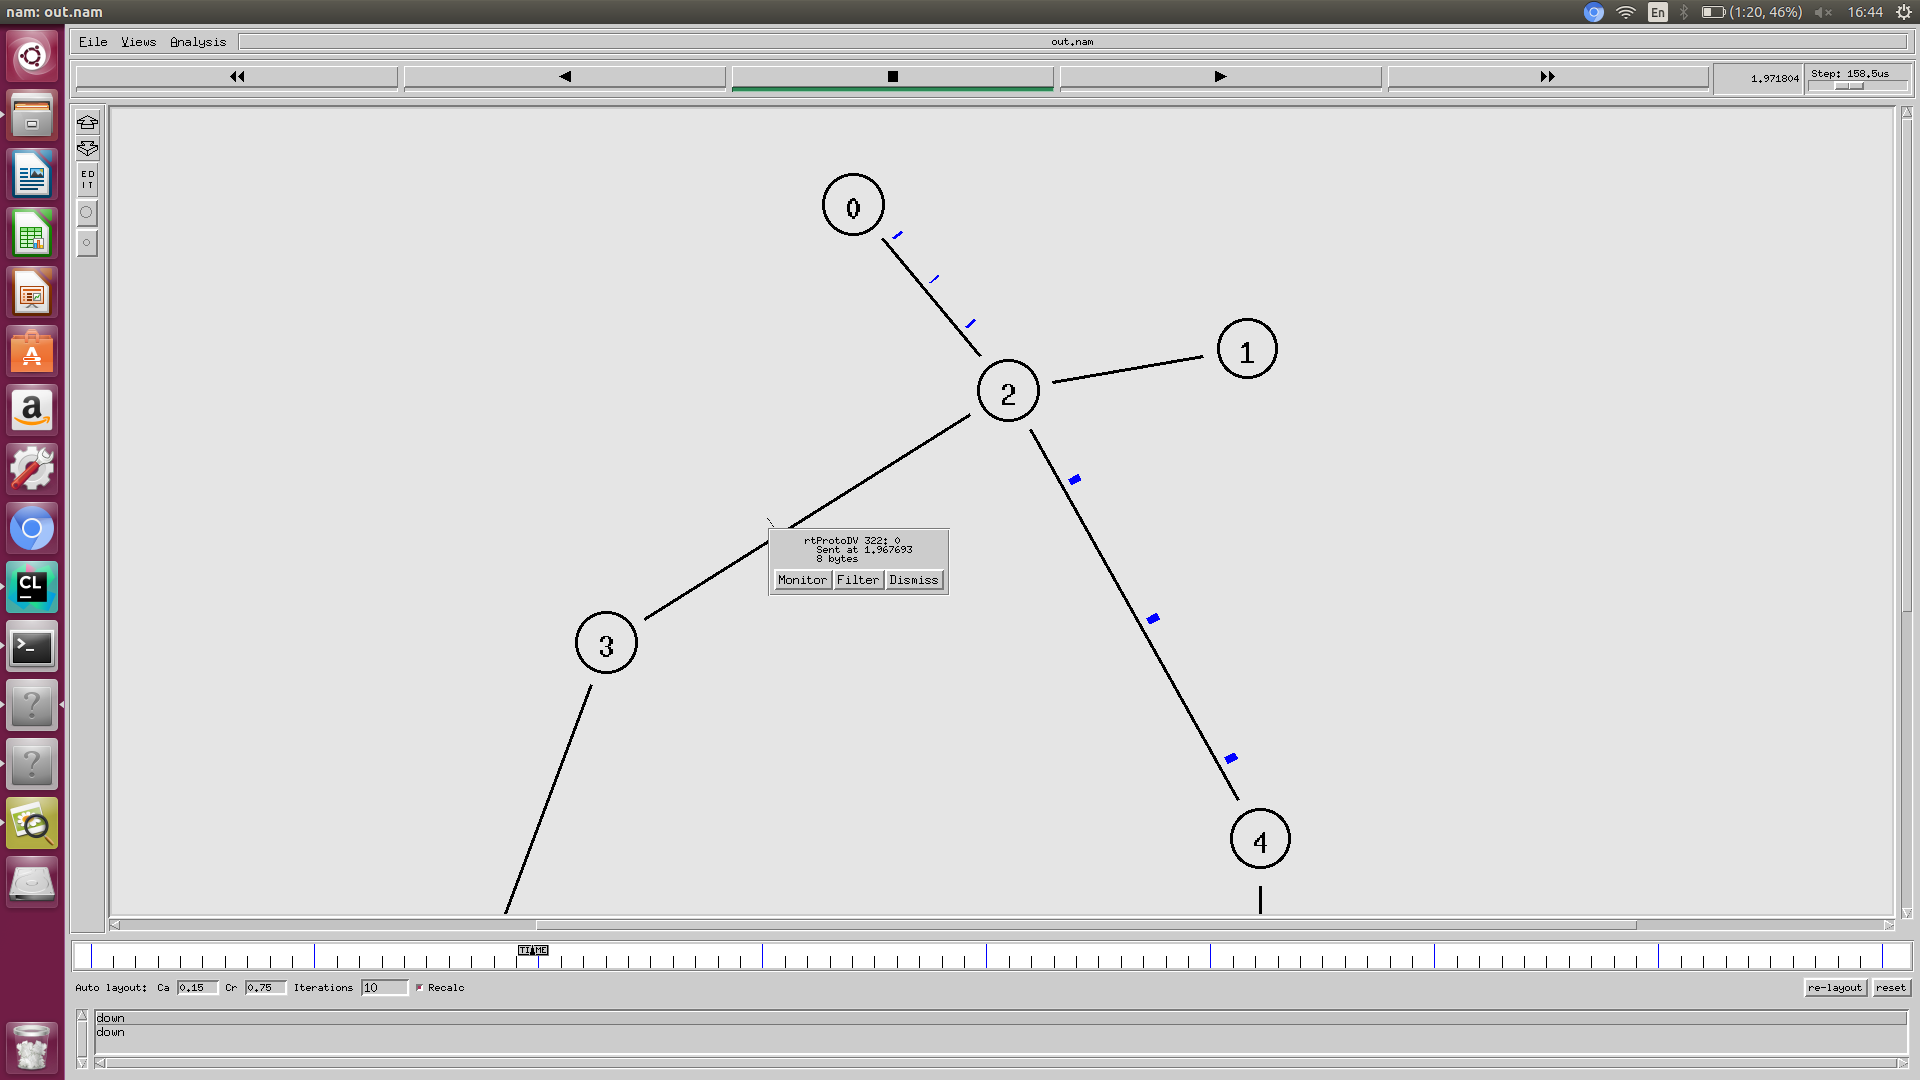
\includegraphics[width=0.99\columnwidth]{tp2-1-DV-1-period.png}
    \caption{Paquets périodiques pour le routage}
    \end{figure}
    
    \begin{figure}
    \centering
    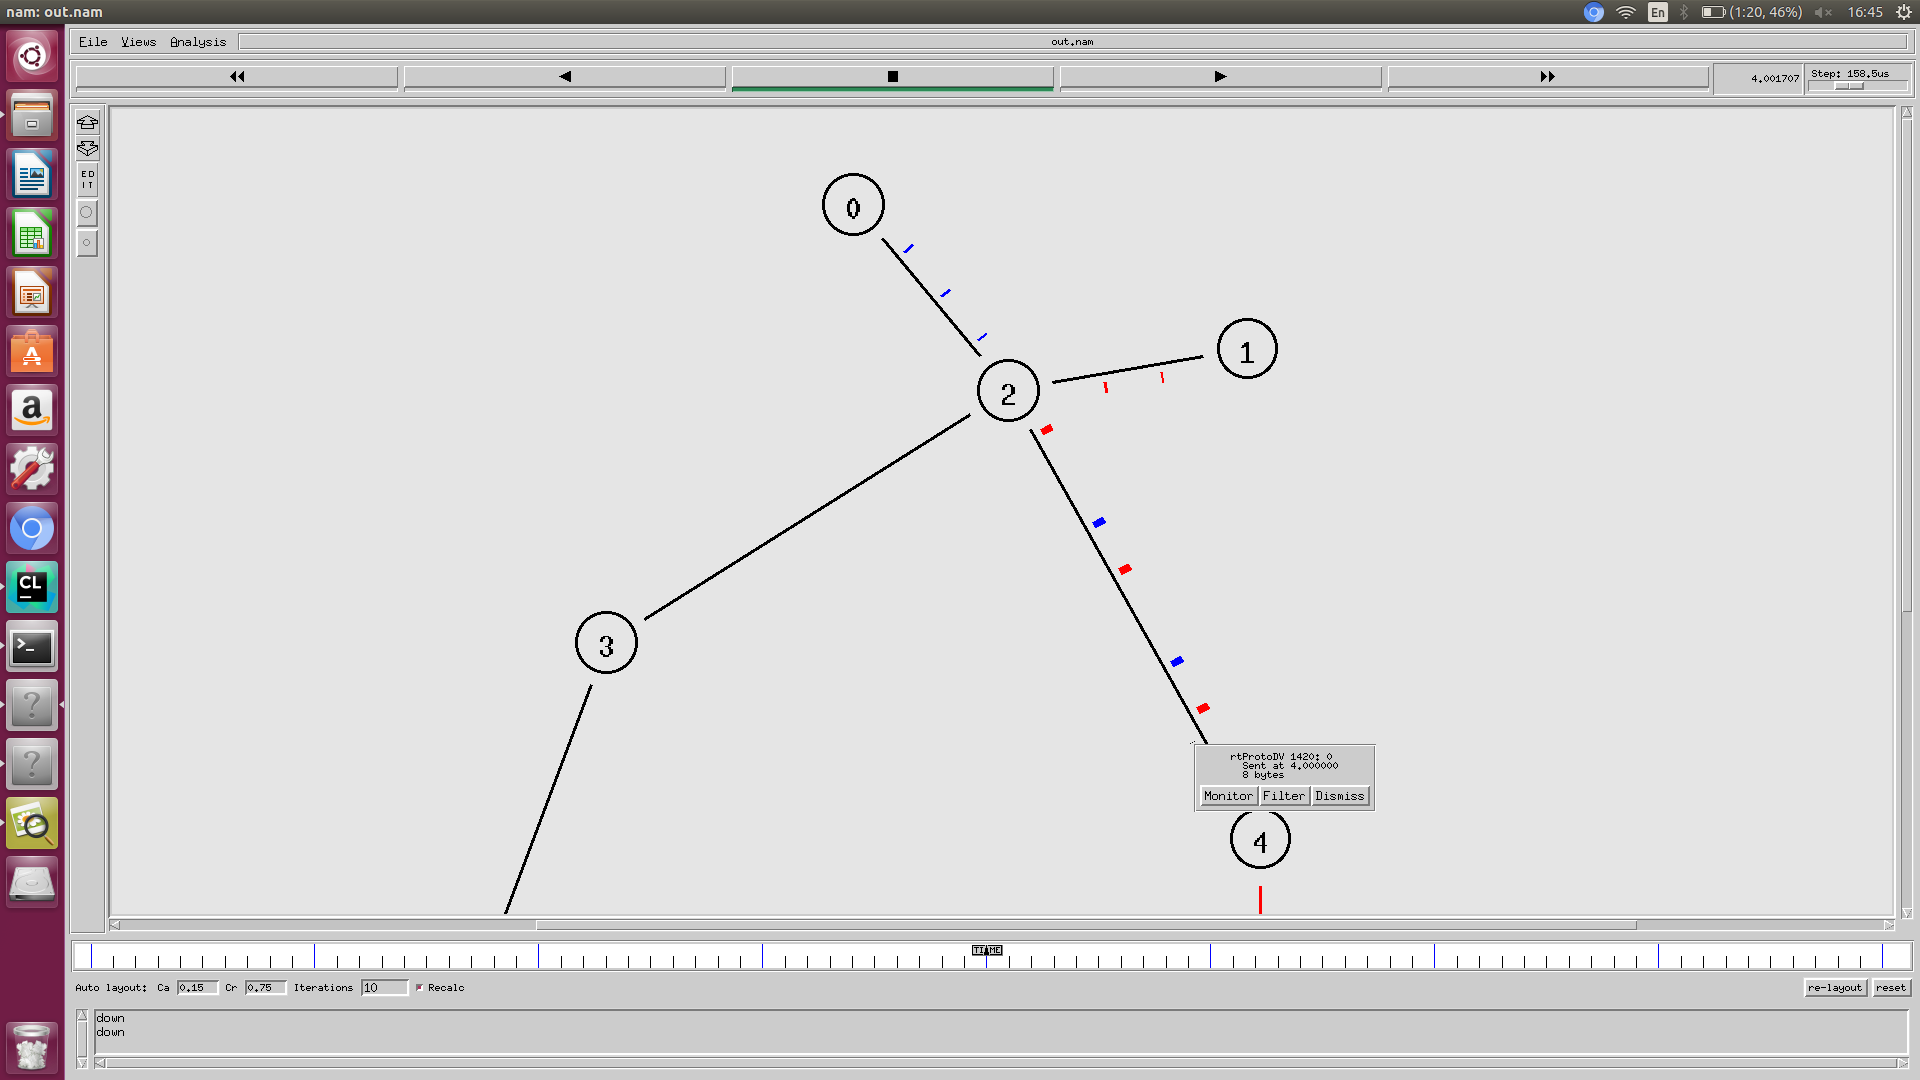
\includegraphics[width=0.99\columnwidth]{tp2-1-DV-2-cut.png}
    \caption{Moment après la rupture}
    \end{figure}
    
    \begin{figure}
    \centering
    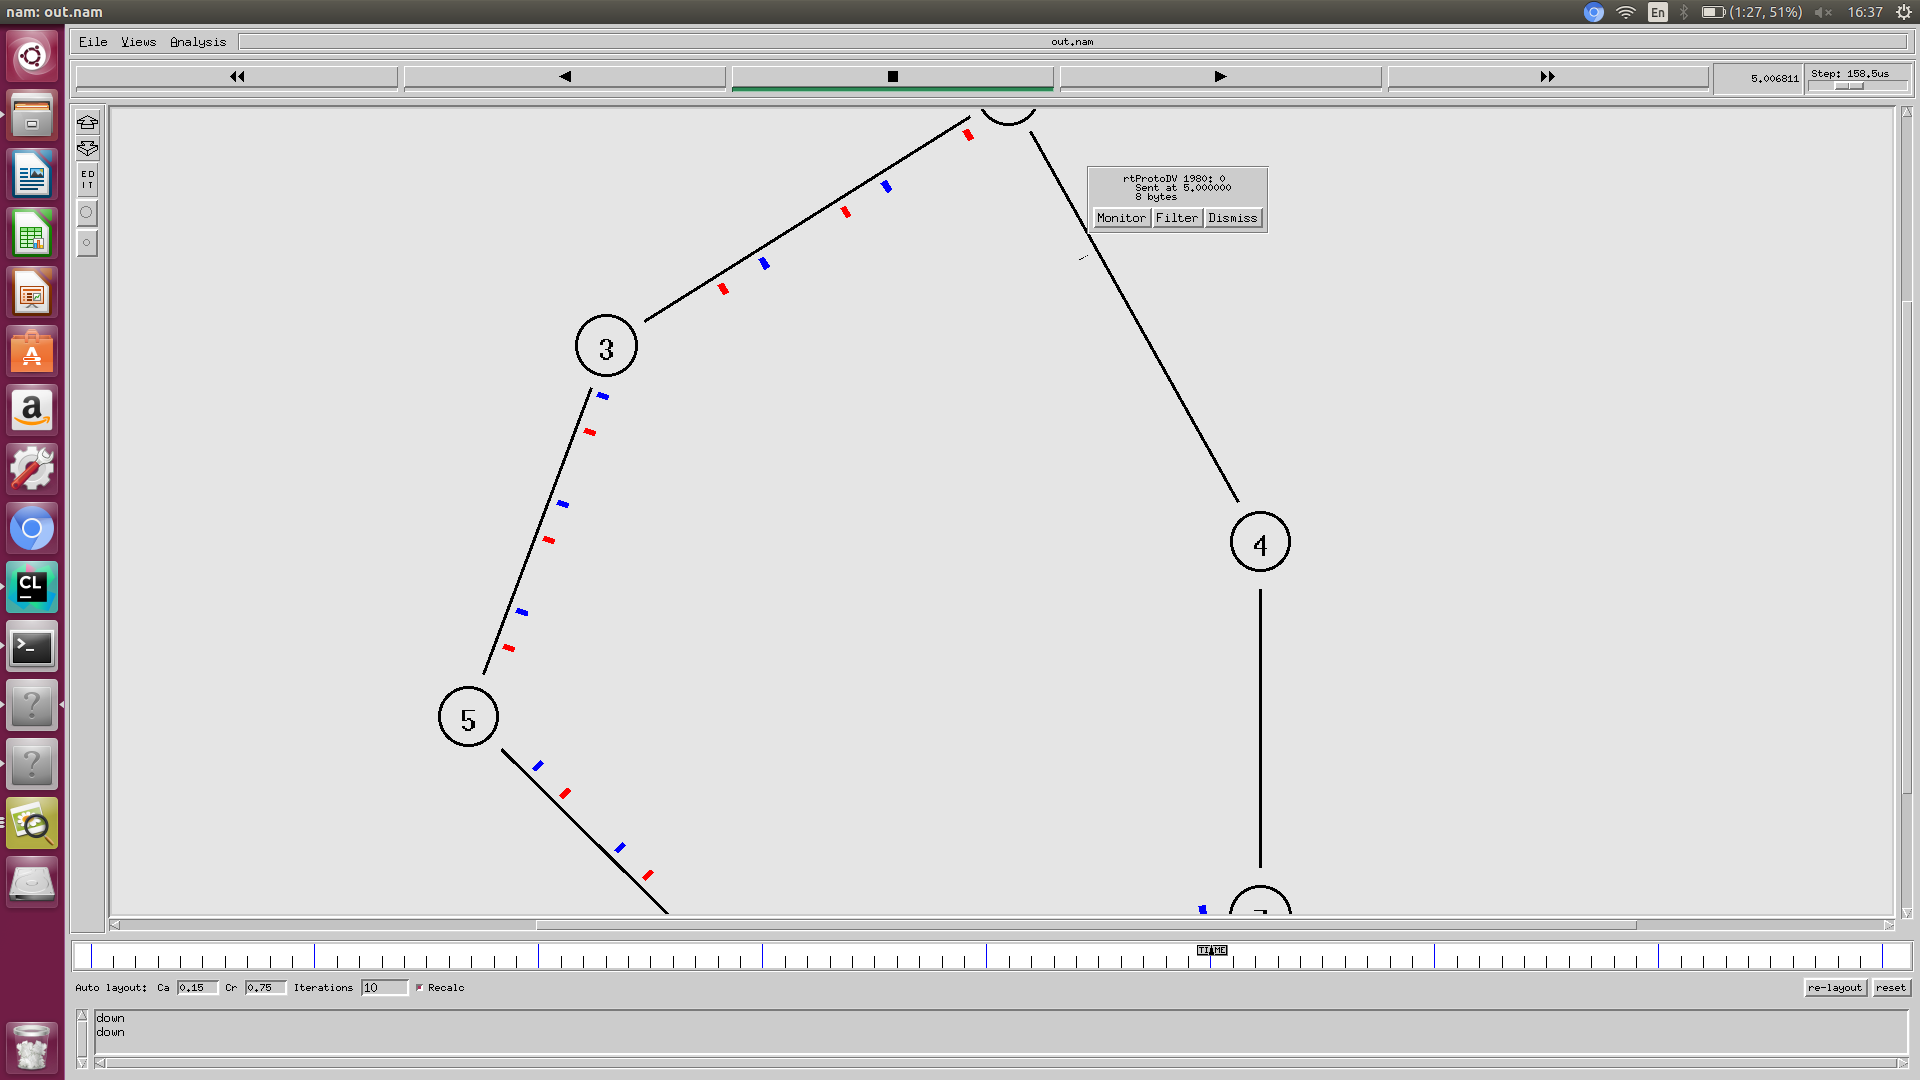
\includegraphics[width=0.99\columnwidth]{tp2-1-DV-4-relink.png}
    \caption{Moment après le rétablissement de la jonction}
    \end{figure}
    
    \begin{figure}
    \centering
    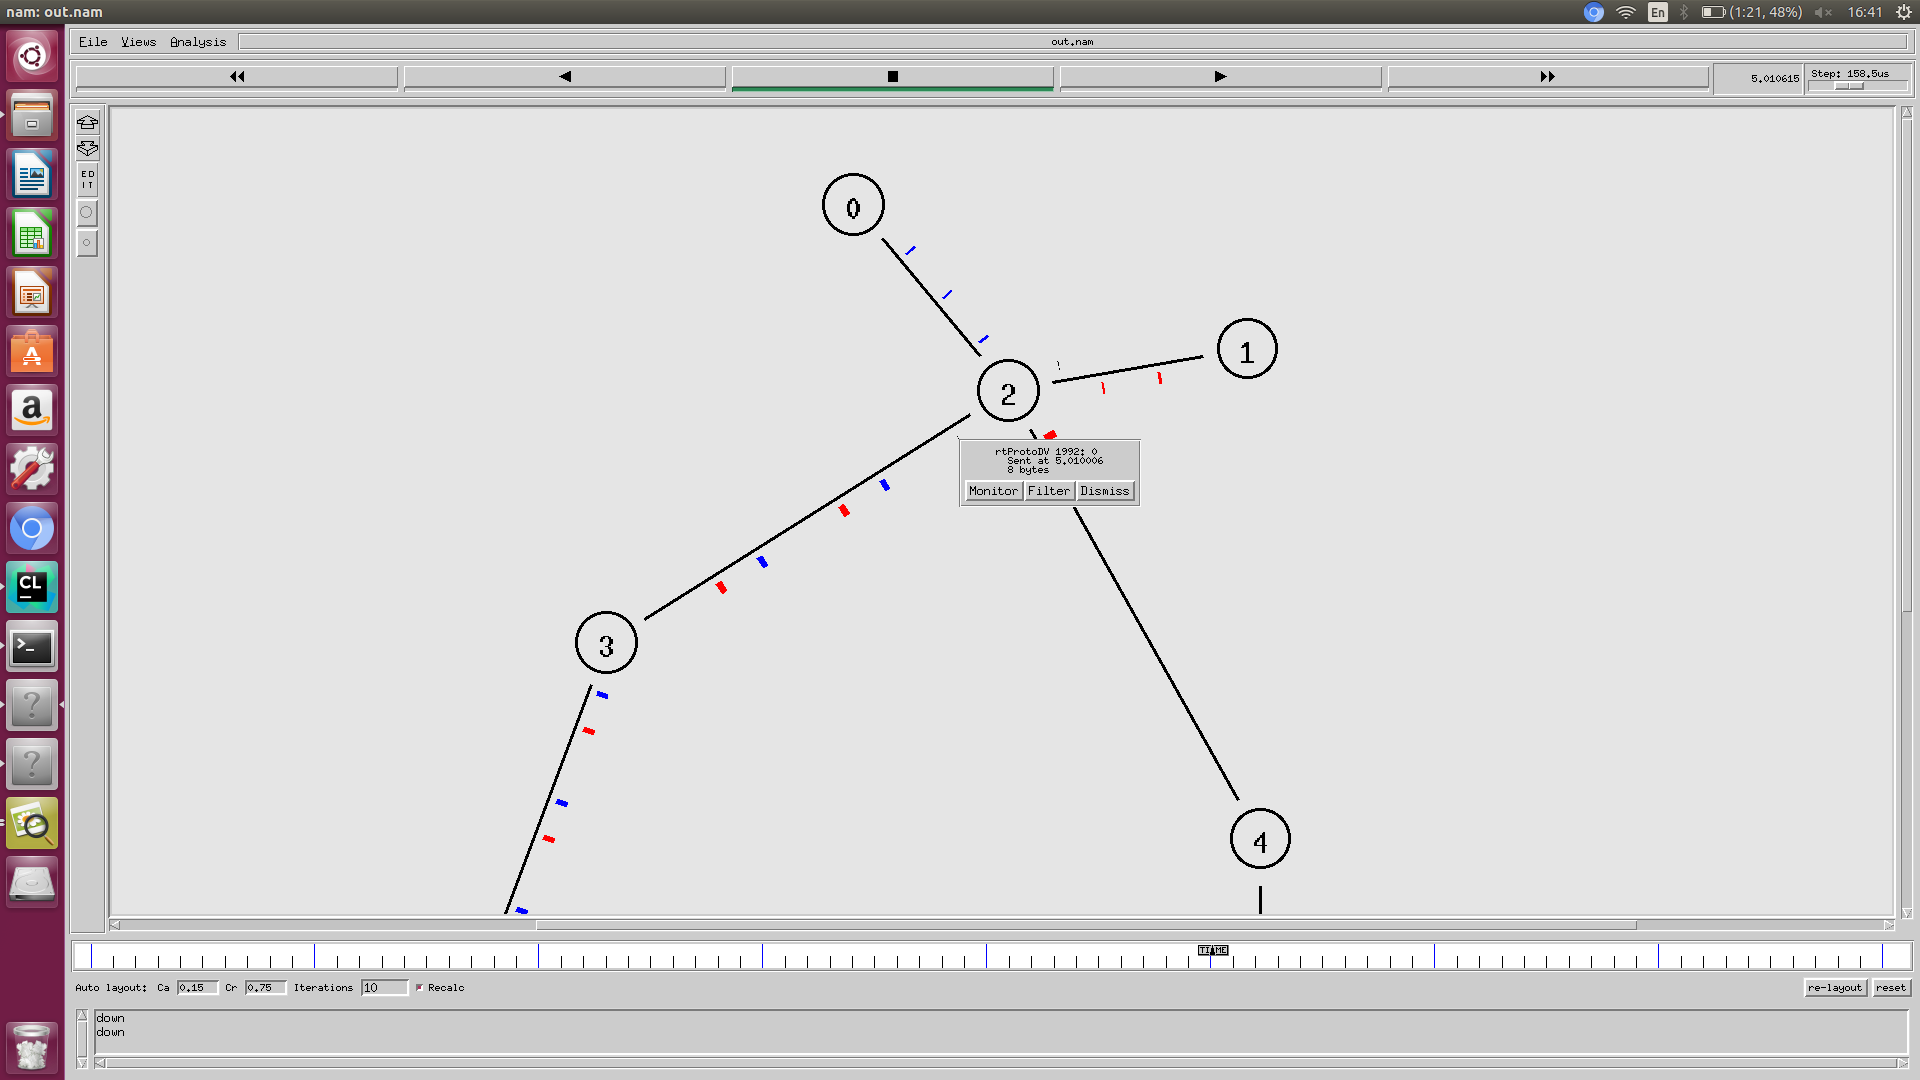
\includegraphics[width=0.99\columnwidth]{tp2-1-DV-5-relink_triggered.png}
    \caption{Routage refait après le rétablissement de la jonction}
    \end{figure}
    
    \begin{figure}
    \centering
    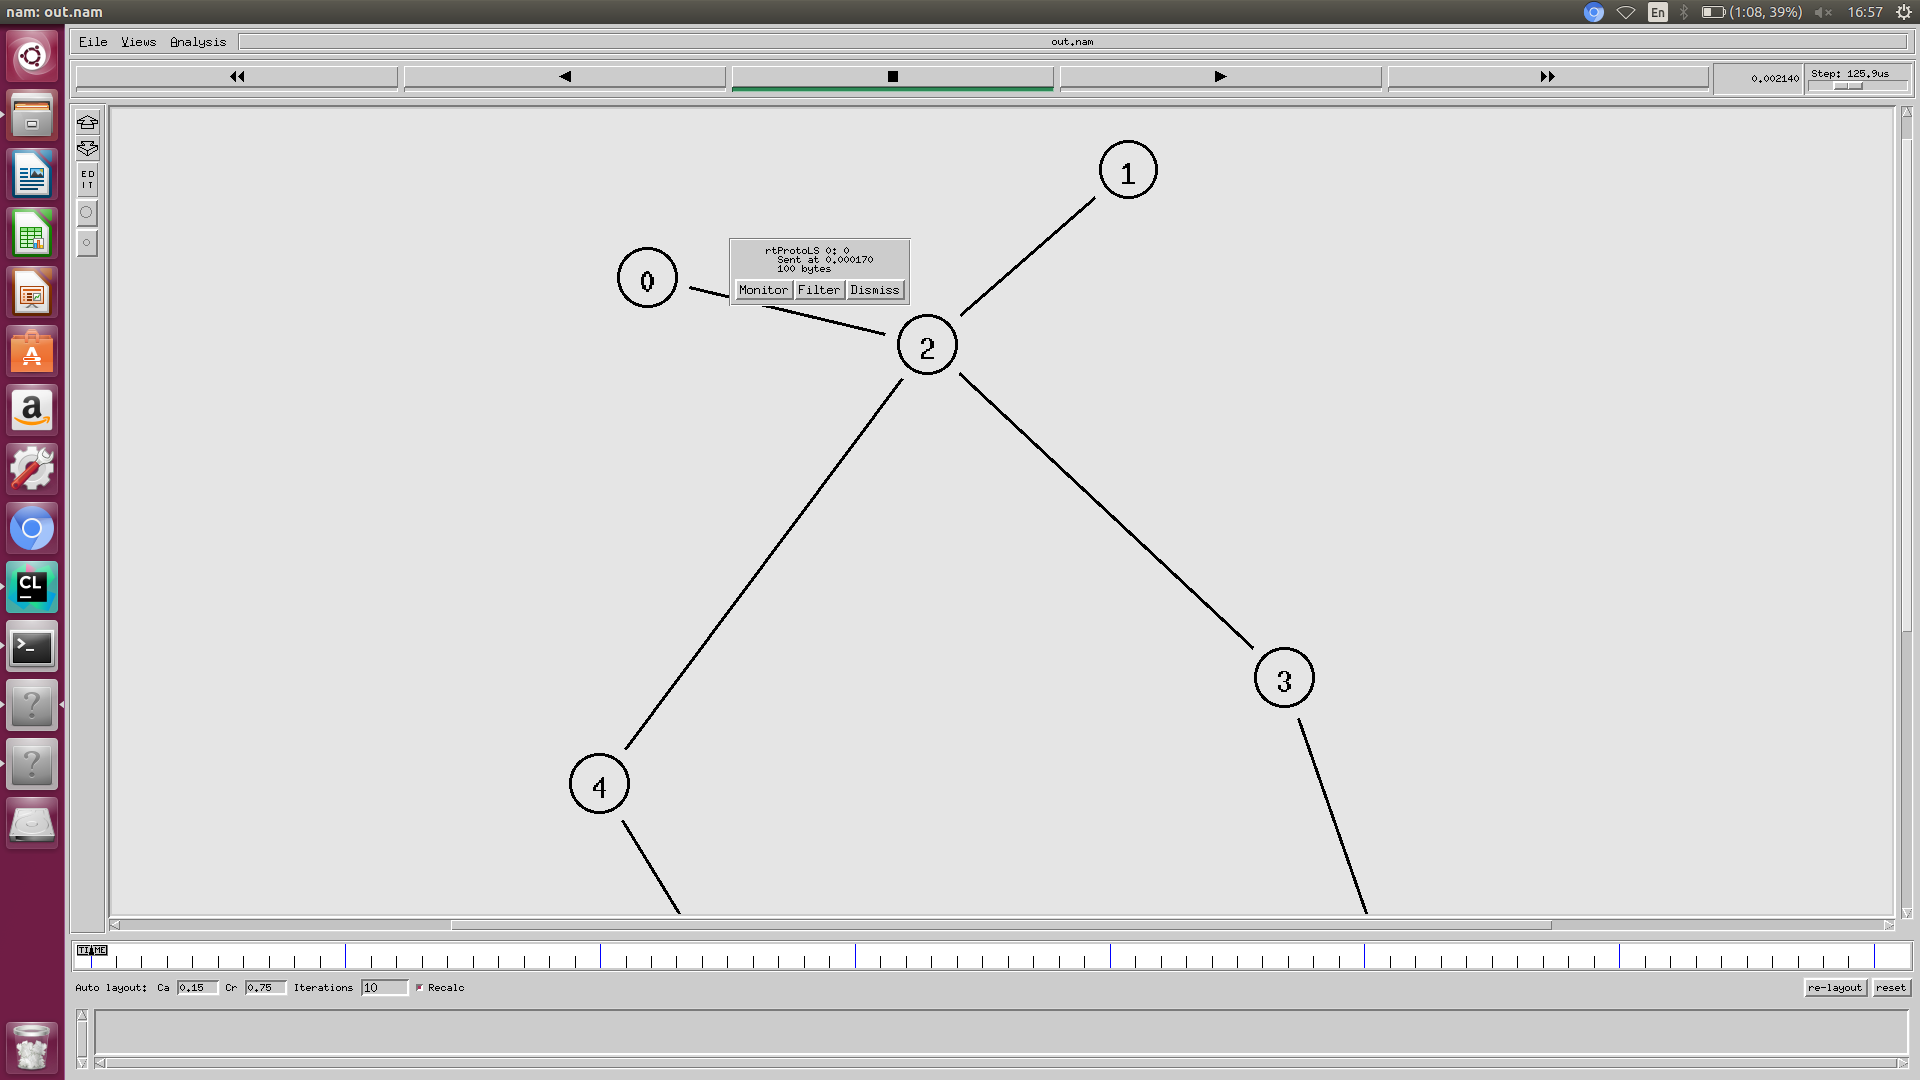
\includegraphics[width=0.99\columnwidth]{tp2-1-LS-0-init.png}
    \caption{Paquets d'initialisation}
    \end{figure}
    \begin{figure}
    \centering
    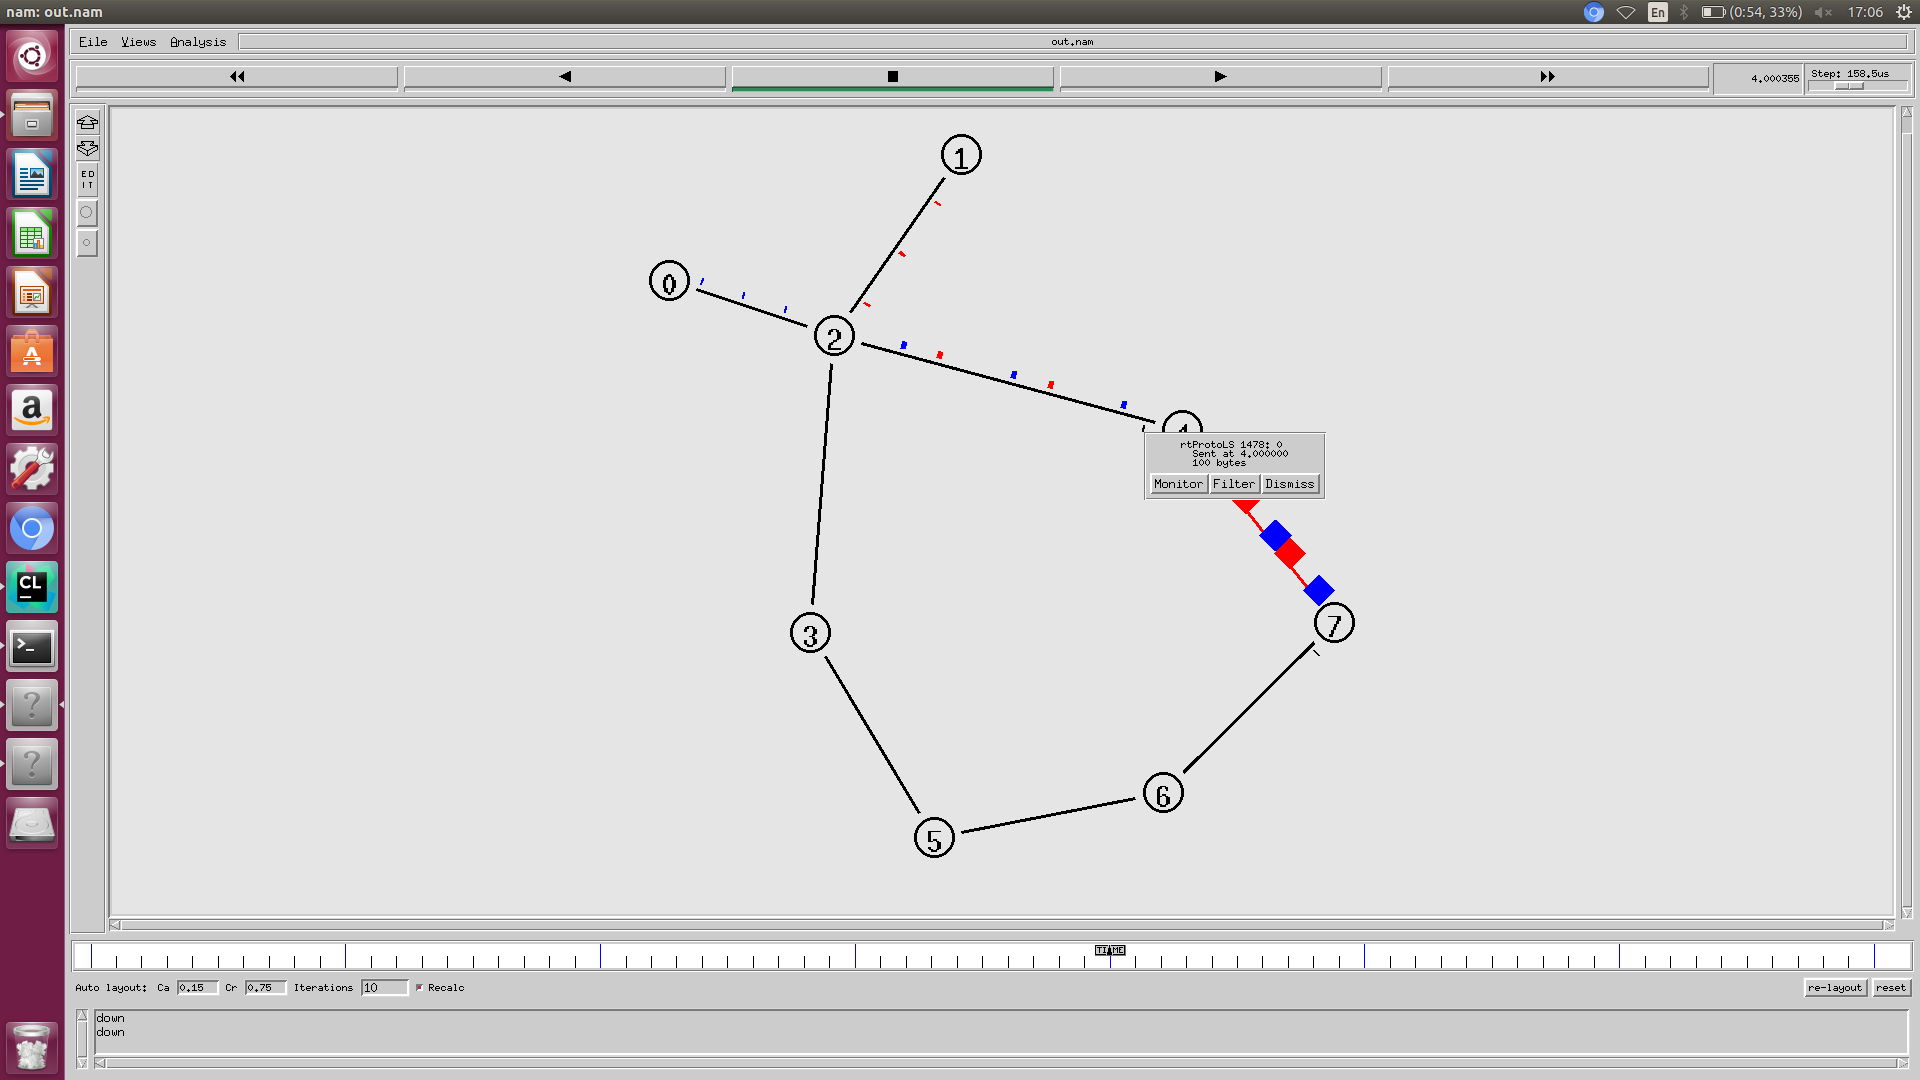
\includegraphics[width=0.99\columnwidth]{tp2-1-LS-1-cut.png}
    \caption{Après la rupture de la jonction}
    \end{figure}
    \begin{figure}
    \centering
    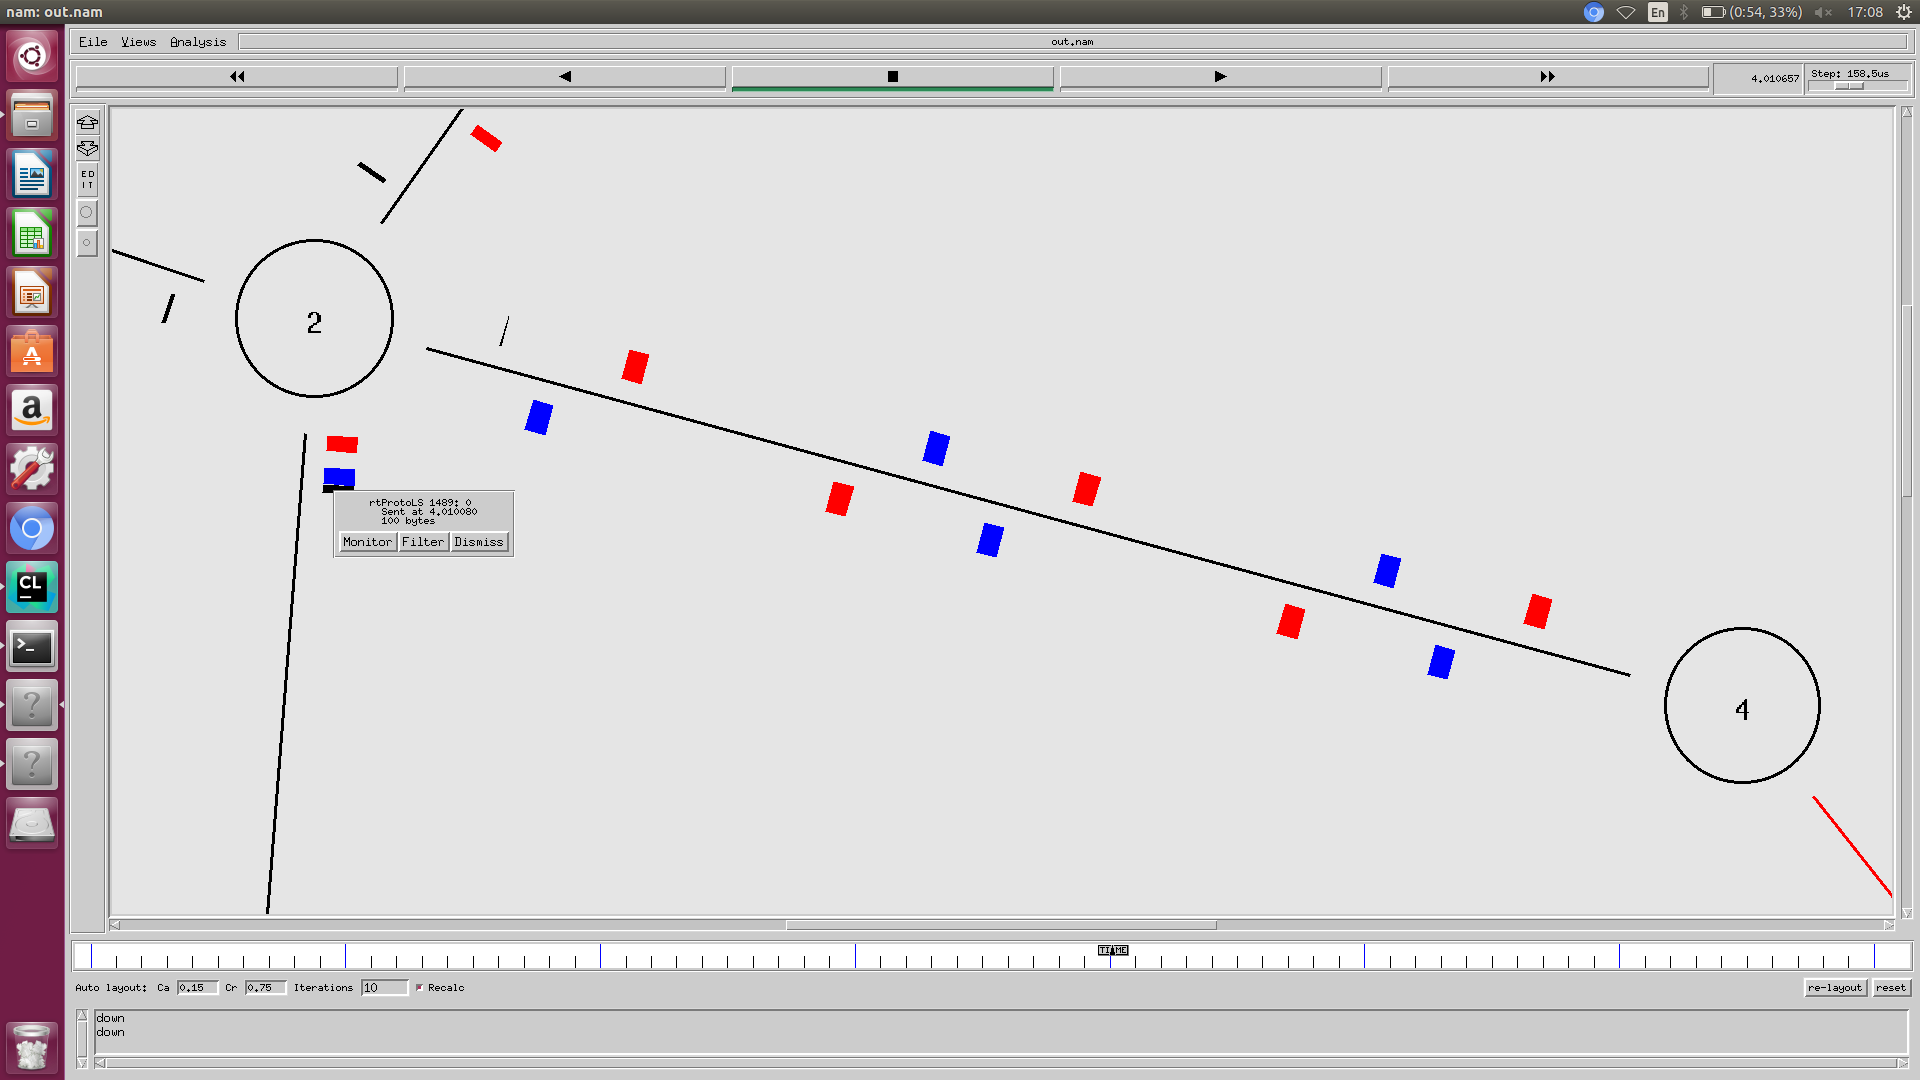
\includegraphics[width=0.99\columnwidth]{tp2-1-LS-2-cut_riggered.png}
    \caption{Routage refait après la rupture}
    \end{figure}
    \begin{figure}
    \centering
    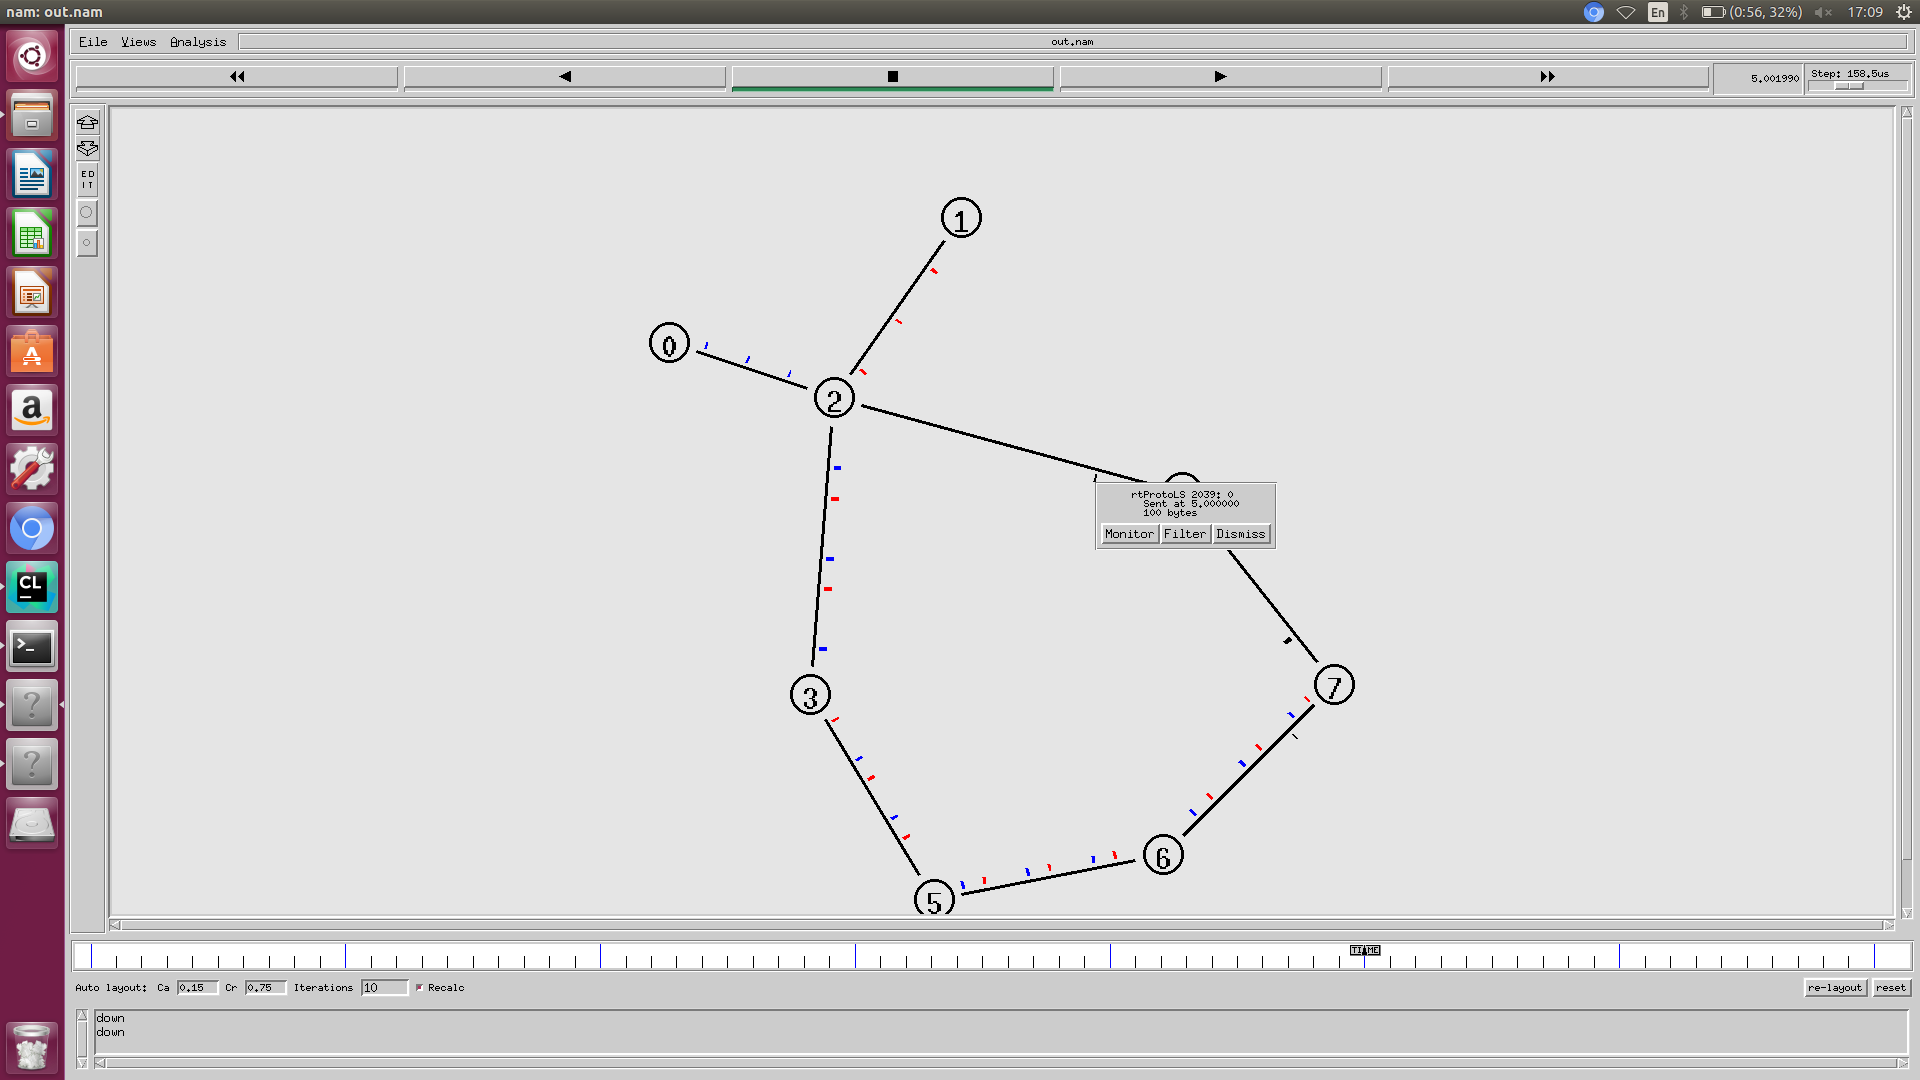
\includegraphics[width=0.99\columnwidth]{tp2-1-LS-3-relink.png}
    \caption{Rétablissement de la jonction}
    \end{figure}
    \begin{figure}
    \centering
    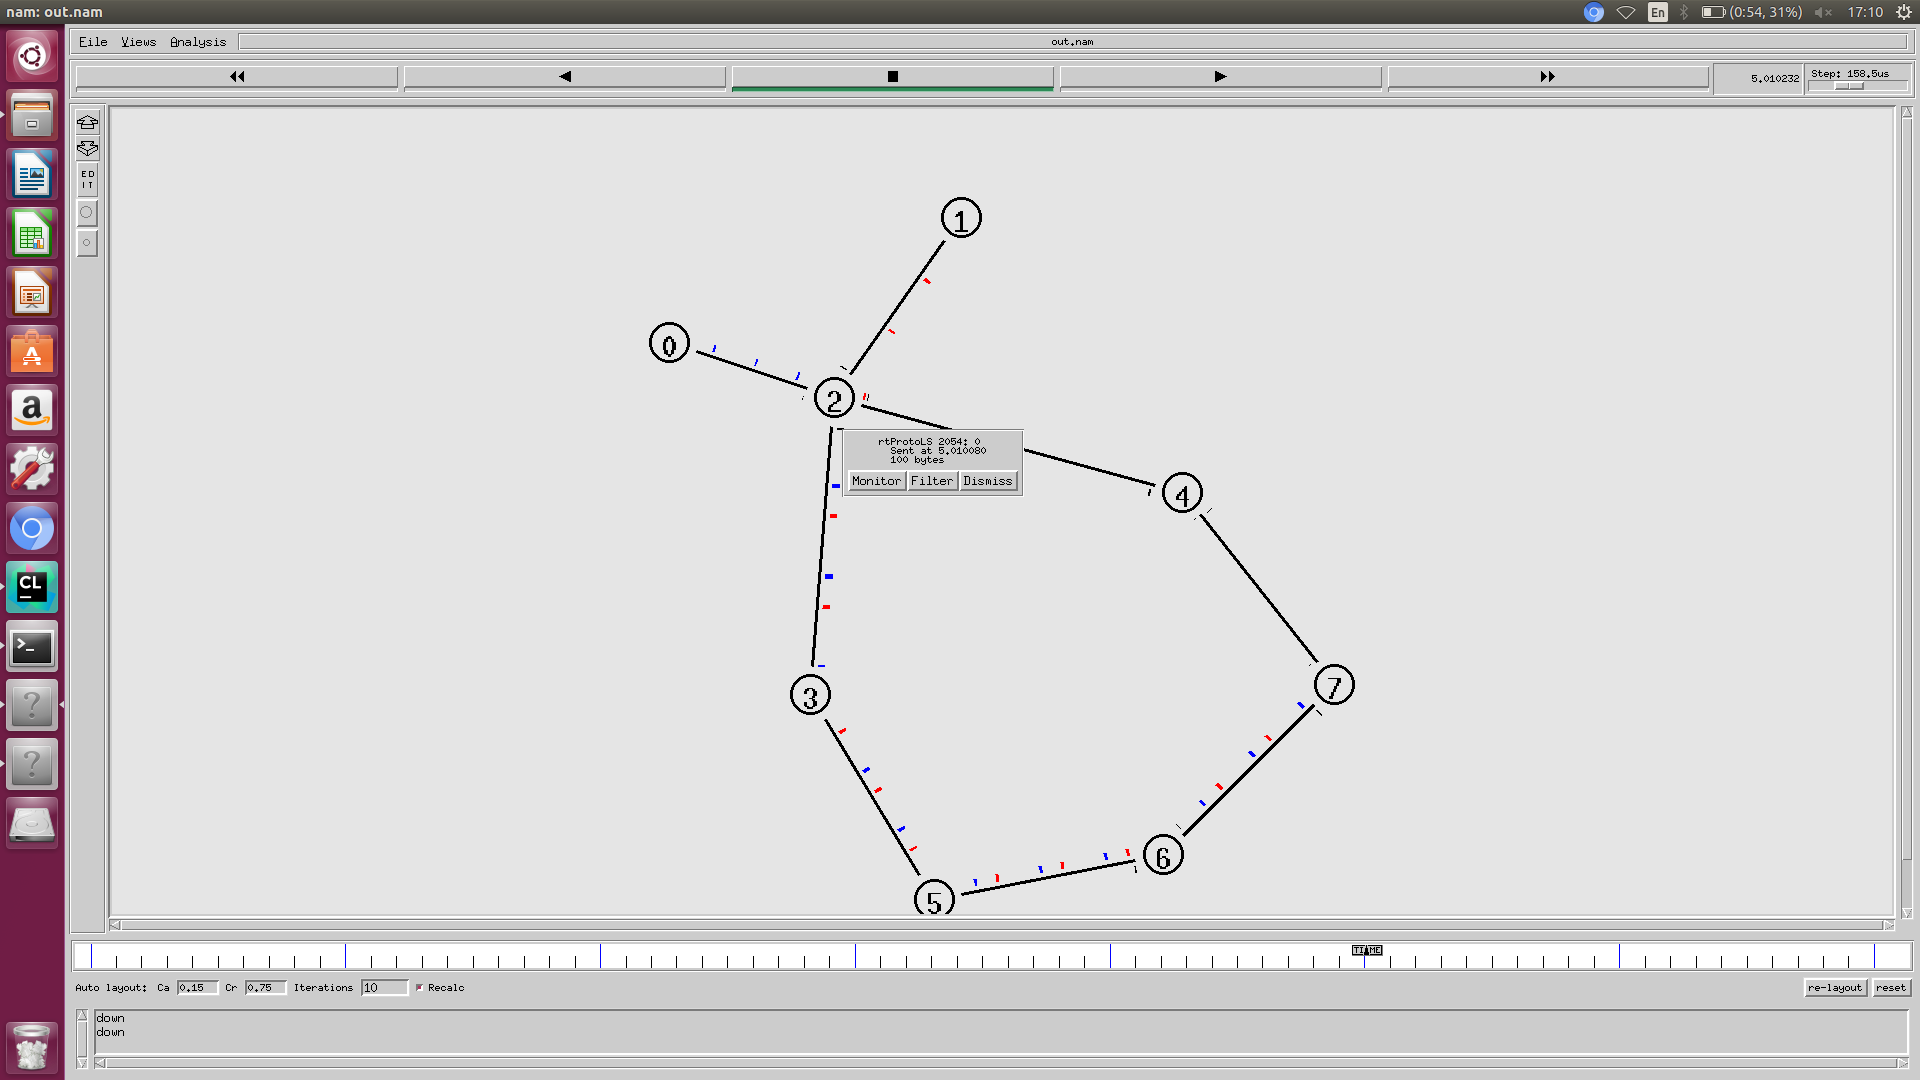
\includegraphics[width=0.99\columnwidth]{tp2-1-LS-4-relink_triggered.png}
    \caption{Routage refait après le rétablissement de la jonction}
    \end{figure}
    \clearpage
    \section{TP3 : Outil de simulation de réseaux : NS-2}
    Afin de mieux expliquer le fonctionnement du code proposé, on a commenté le plus de lignes possibles afin de clarifier directement les lignes qui sont découvertes à ce moment. Ainsi, le gros de ce TP se passe principalement dans le code en annexe. Les couleurs ont été rajoutés au sein de la procédure attach-expo-traffic.
    
    La procédure attach-expo-traffic permet comme son nom l'indique d'attacher aux noeuds 0, 1 et 2 les sources de trafic exponentielles. Celle-ci crée un agent UDP auxquels elle attache simultanément l'agent source de trafic, mais aussi un agent permettant de recevoir ce trafic (LossMonitor). Elle est appelée pour les trois noeuds qui génèreront du trafic, afin de ne pas répéter le code.
    
    La procédure record convertit ce que les "sink" recoivent en octets afin de les écrire dans les fichiers f0, f1 et f2, puis se rappelle après un certain temps afin de continuer l'enregistrement, en remettant les variables contenant les octets à 0.

    En changeant le temps d'enregistrement des courbes nous obtenons un taux d'échantillonage plus ou moins élevé. Cela nous permet de voir qu'en ayant un taux d'échantillonage trop bas, on a un résultat qui n'est pas exactement la réalité. Le débit ne réduit pas, il s'arrête à certains moments. Ainsi un taux d'échantillonnage de 0,1s, c'est-à-dire le délai impliqué par les connexions, on peut voir les trafics démarrer et s'arrêter, plutôt que réduire et se modifier. On a donc un résultat plus proche de la réalité.
    \clearpage
    \begin{figure}
      \centering
        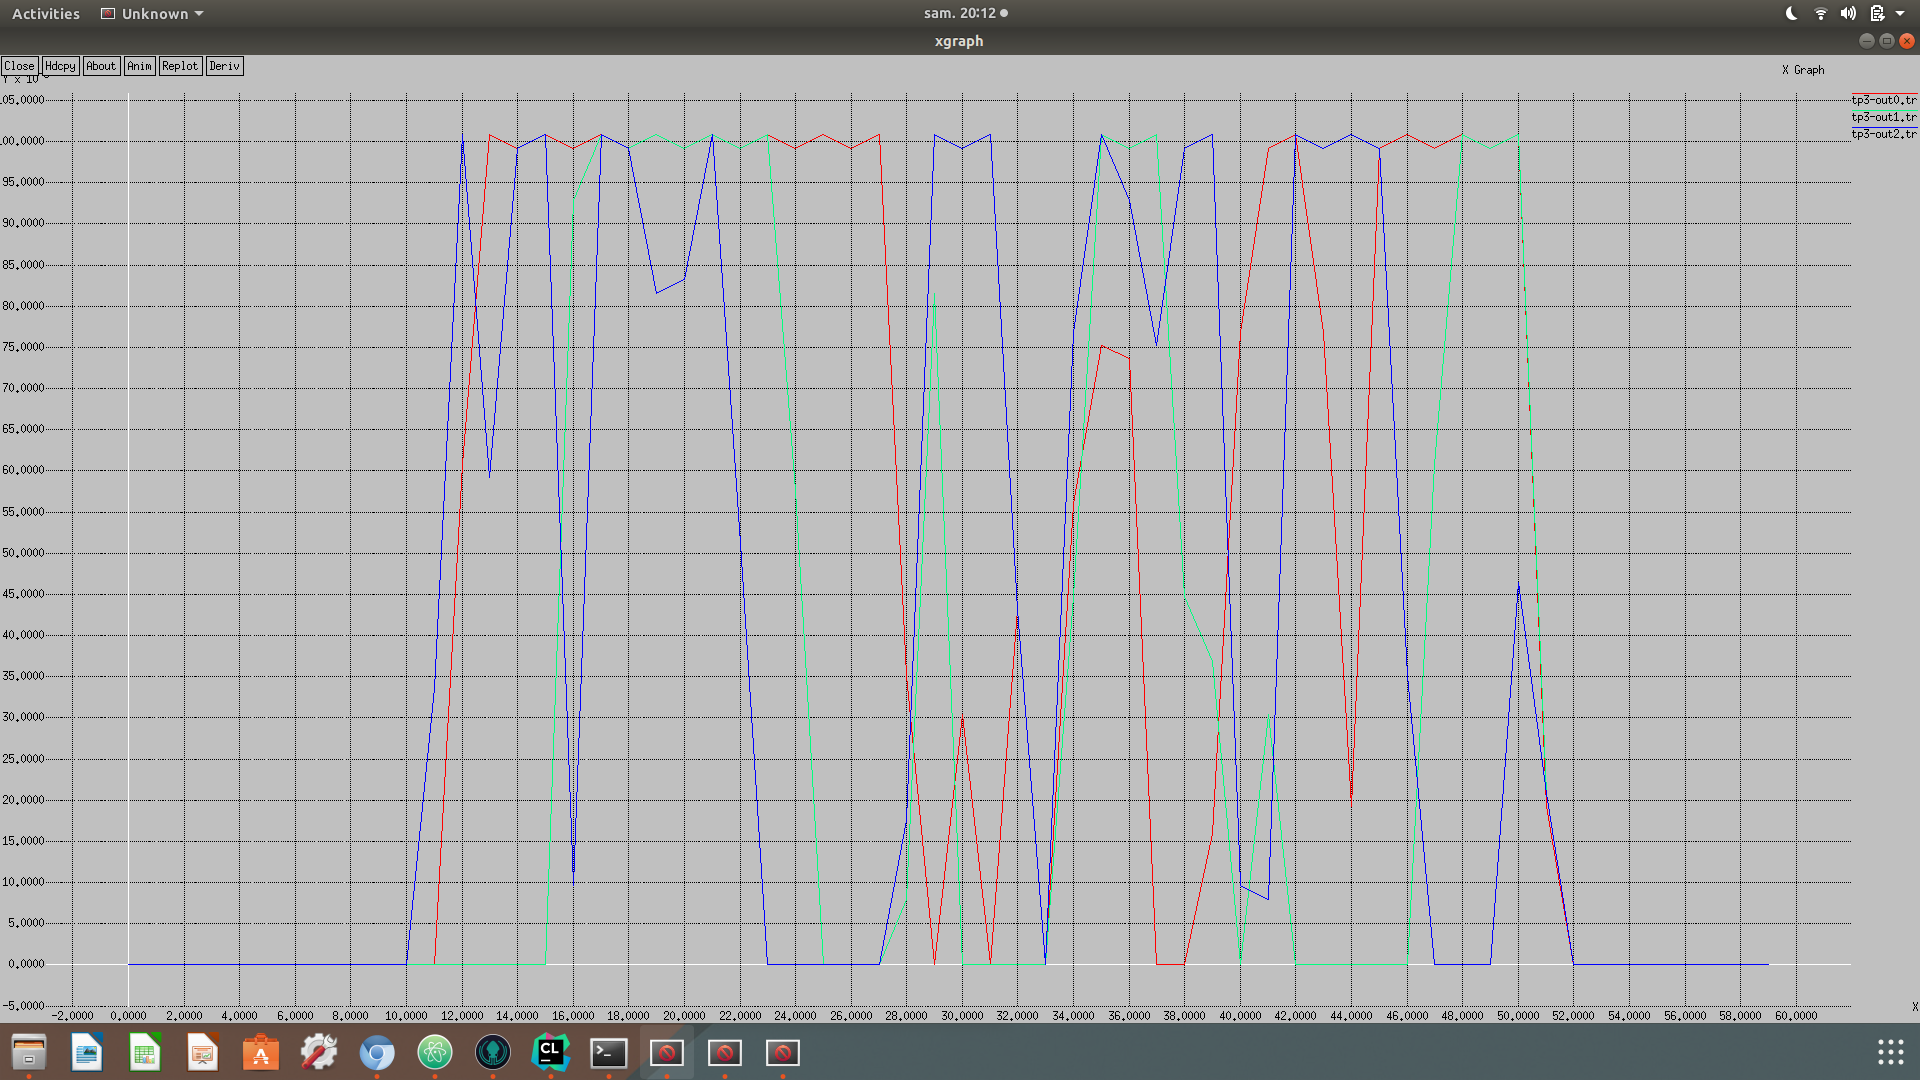
\includegraphics[width=0.99\columnwidth]{1,0.png}
        \caption{xGraph : Échantillonage de 1 seconde}
    \end{figure}

    \begin{figure}
      \centering
        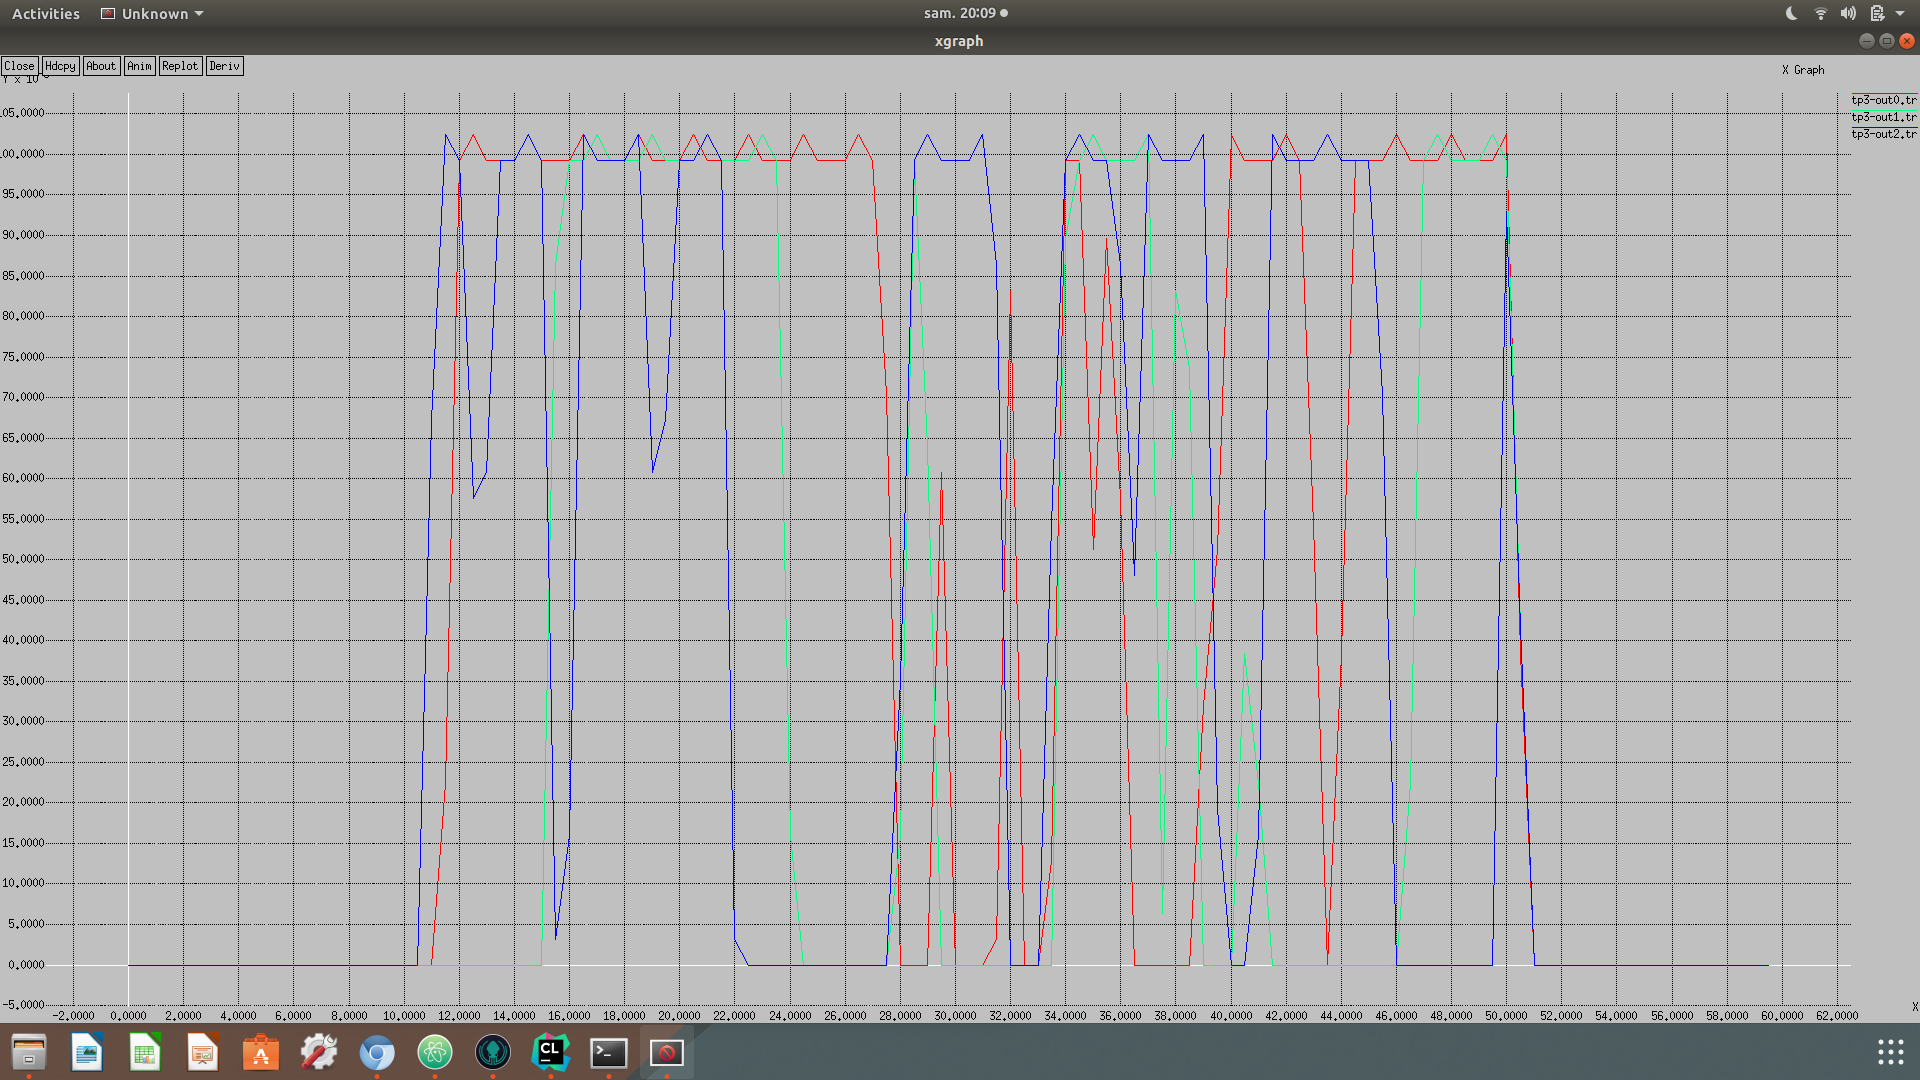
\includegraphics[width=0.99\columnwidth]{0,5.png}
        \caption{xGraph : Échantillonage de 0.5 seconde}
    \end{figure}

    \begin{figure}
      \centering
        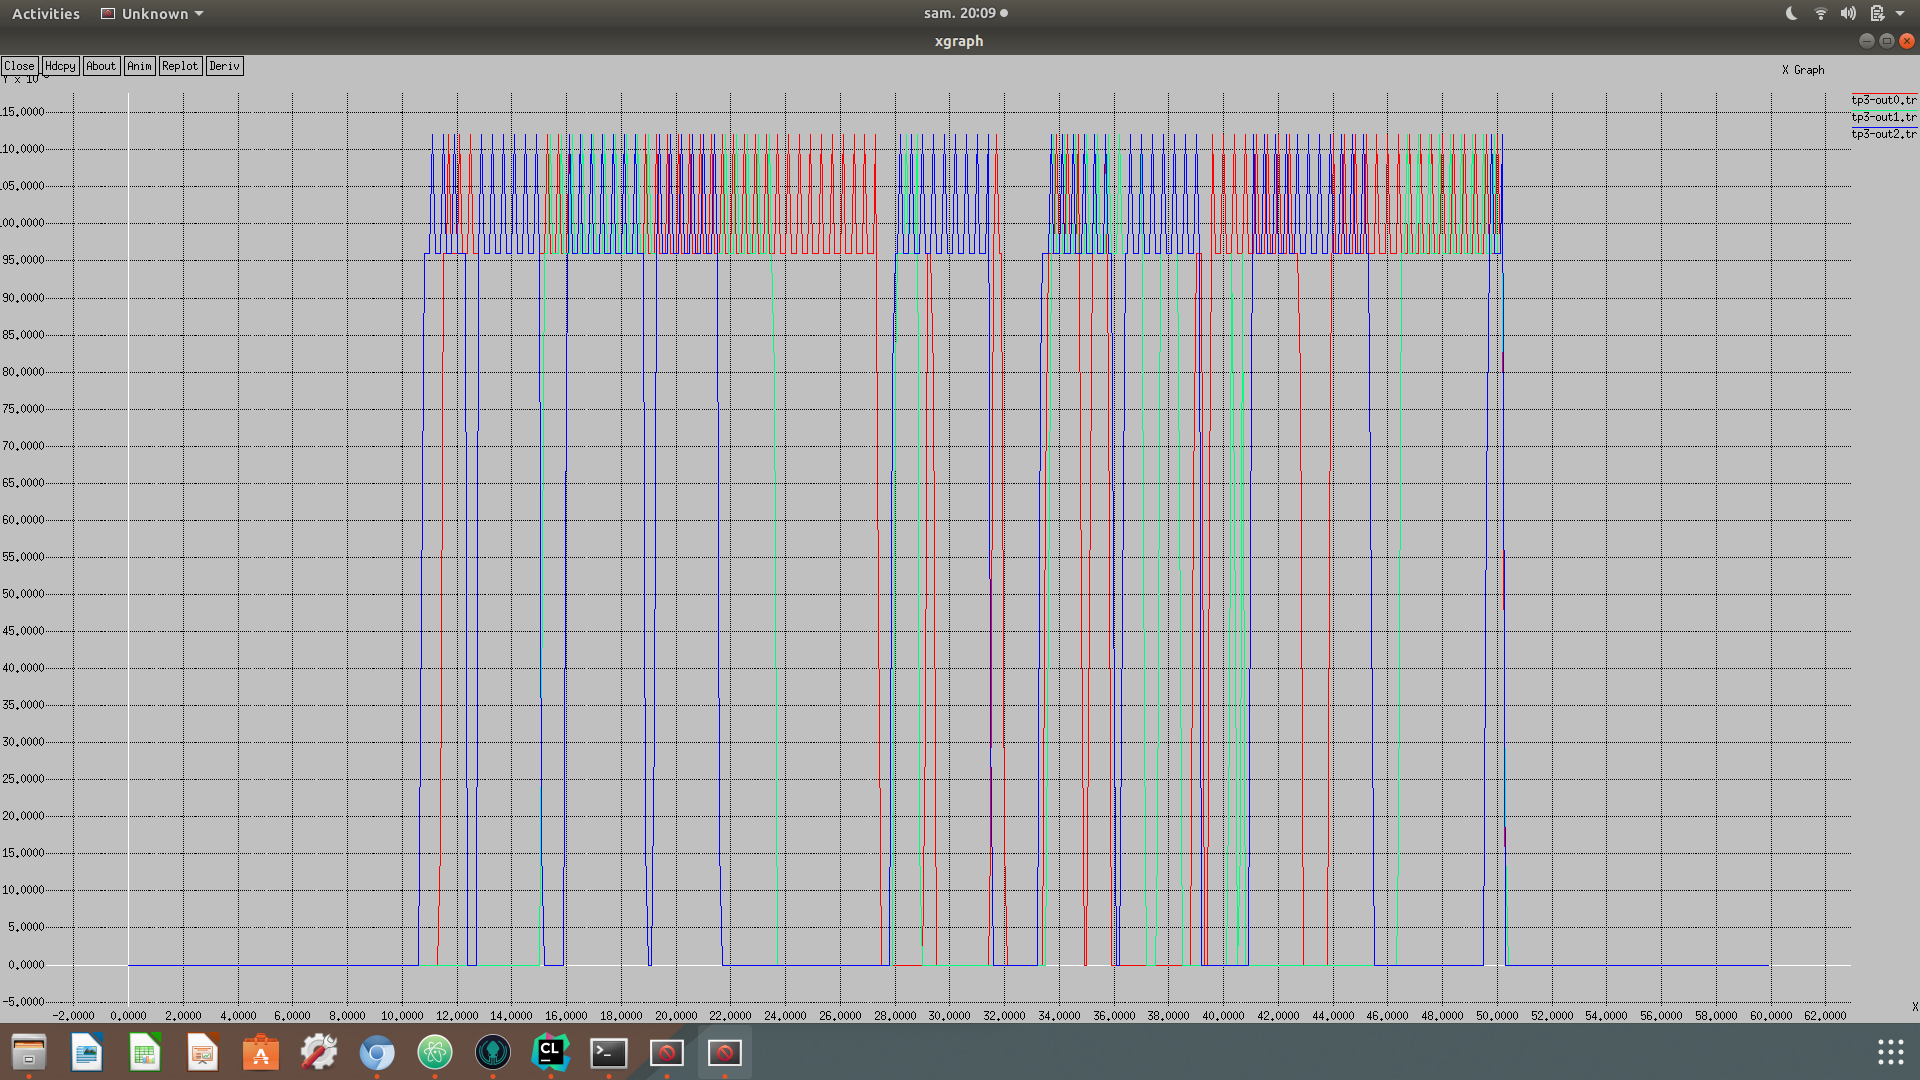
\includegraphics[width=0.99\columnwidth]{0,1.png}
        \caption{xGraph : Échantillonage 0.1 seconde}
    \end{figure}

\end{document}
